\documentclass[border=3pt]{standalone}
\usepackage{tikz}
\usetikzlibrary{positioning, arrows.meta, shapes.geometric, fit,
                 decorations.pathreplacing, calc, backgrounds}
\usepackage{amsmath,amssymb}

\definecolor{localblue}{HTML}{4393C3}
\definecolor{globalorange}{HTML}{E66101}
\definecolor{innovgreen}{HTML}{1B7837}
\definecolor{readoutpurple}{HTML}{7B3294}
\definecolor{inputgray}{HTML}{D9D9D9}
\definecolor{bgblue}{HTML}{DEEBF7}
\definecolor{bgorange}{HTML}{FEE6CE}
\definecolor{bggreen}{HTML}{D5E8D4}

\begin{document}
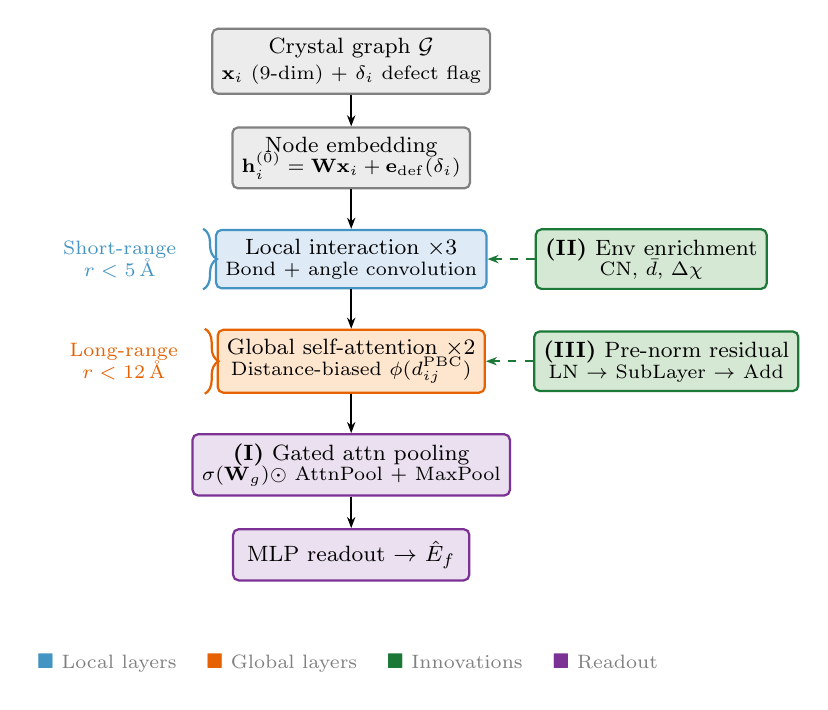
\begin{tikzpicture}[
    node distance=0.5cm and 0.8cm,
    block/.style={draw, rounded corners=2pt, minimum height=0.65cm,
                  minimum width=2.0cm, font=\footnotesize, thick,
                  align=center},
    localblock/.style={block, fill=bgblue, draw=localblue},
    globalblock/.style={block, fill=bgorange, draw=globalorange},
    innovblock/.style={block, fill=bggreen, draw=innovgreen},
    ioblock/.style={block, fill=inputgray!50, draw=gray},
    readblock/.style={block, fill=readoutpurple!15, draw=readoutpurple},
    arrow/.style={-{Stealth[length=4pt]}, thick},
    label/.style={font=\scriptsize, text=gray},
    bracetext/.style={font=\scriptsize, text=gray, align=center},
]

% === Input ===
\node[ioblock, minimum width=3cm] (input) {Crystal graph $\mathcal{G}$\\
  \scriptsize $\mathbf{x}_i$ (9-dim) $+$ $\delta_i$ defect flag};

% === Embedding ===
\node[ioblock, below=0.4cm of input, minimum width=3cm] (embed) {
  Node embedding\\[-2pt]
  \scriptsize $\mathbf{h}_i^{(0)} = \mathbf{W}\mathbf{x}_i + \mathbf{e}_{\mathrm{def}}(\delta_i)$};

% === Local layers ===
\node[localblock, below=0.5cm of embed, minimum width=3cm] (local) {
  Local interaction $\times 3$\\[-2pt]
  \scriptsize Bond + angle convolution};

% === Innovation: Local env enrichment ===
\node[innovblock, right=0.6cm of local, minimum width=2.4cm] (envrich) {
  \textbf{(II)} Env enrichment\\[-2pt]
  \scriptsize CN, $\bar{d}$, $\Delta\chi$};

% === Global layers ===
\node[globalblock, below=0.5cm of local, minimum width=3cm] (global) {
  Global self-attention $\times 2$\\[-2pt]
  \scriptsize Distance-biased $\phi(d_{ij}^{\mathrm{PBC}})$};

% === Innovation: Pre-norm ===
\node[innovblock, right=0.6cm of global, minimum width=2.4cm] (prenorm) {
  \textbf{(III)} Pre-norm residual\\[-2pt]
  \scriptsize LN $\to$ SubLayer $\to$ Add};

% === Innovation: Gated pooling ===
\node[readblock, below=0.5cm of global, minimum width=3cm] (pool) {
  \textbf{(I)} Gated attn pooling\\[-2pt]
  \scriptsize $\sigma(\mathbf{W}_g) \odot$ AttnPool $+$ MaxPool};

% === MLP head ===
\node[readblock, below=0.4cm of pool, minimum width=3cm] (mlp) {
  MLP readout $\to$ $\hat{E}_f$};

% === Arrows ===
\draw[arrow] (input)  -- (embed);
\draw[arrow] (embed)  -- (local);
\draw[arrow] (local)  -- (global);
\draw[arrow] (global) -- (pool);
\draw[arrow] (pool)   -- (mlp);

% Innovation arrows
\draw[arrow, innovgreen, dashed] (envrich) -- (local);
\draw[arrow, innovgreen, dashed] (prenorm) -- (global);

% === Side braces ===
\draw[decorate, decoration={brace, amplitude=5pt, mirror},
      localblue, thick]
  ($(local.south west) + (-0.15, 0)$) --
  ($(local.north west) + (-0.15, 0)$)
  node[midway, left=6pt, bracetext, text=localblue]
  {Short-range\\$r < 5$\,\AA};

\draw[decorate, decoration={brace, amplitude=5pt, mirror},
      globalorange, thick]
  ($(global.south west) + (-0.15, 0)$) --
  ($(global.north west) + (-0.15, 0)$)
  node[midway, left=6pt, bracetext, text=globalorange]
  {Long-range\\$r < 12$\,\AA};

% === Legend ===
\node[below=0.8cm of mlp, font=\scriptsize, text=gray, align=center] (legend) {
  \textcolor{localblue}{$\blacksquare$} Local layers \quad
  \textcolor{globalorange}{$\blacksquare$} Global layers \quad
  \textcolor{innovgreen}{$\blacksquare$} Innovations \quad
  \textcolor{readoutpurple}{$\blacksquare$} Readout
};

\end{tikzpicture}
\end{document}
